\section{System Implementation} 
hue hue hue

\subsection{Gesture Recognition}
\subsubsection{Preprocessing}
Once the acceleration and rotation data is sent from the device to the computer,
 the values are smoothed with an average of the 20 previous values in order to avoid and reduce the effect of noise on the sensors.
 This phase is called preprocessing of the data. 
 This allowed us to have more precise information, as can be deducted from the images  \ref{fig:figure2} and \ref{fig:figure3}

\begin{figure}[!h]
\centering
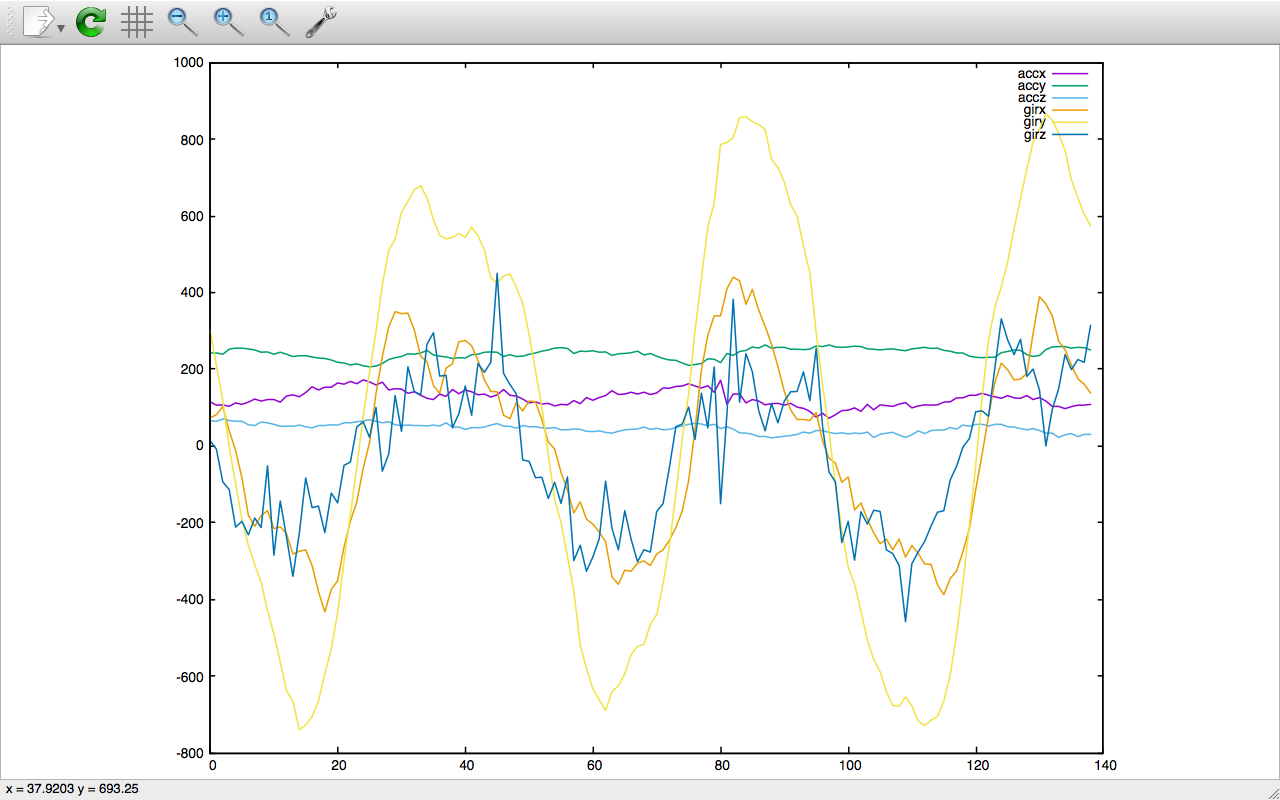
\includegraphics[width=0.9\columnwidth]{img/raw}
\caption{Data from the device before preprocessing.}
\label{fig:figure2}
\end{figure}

\begin{figure}[!h]
\centering
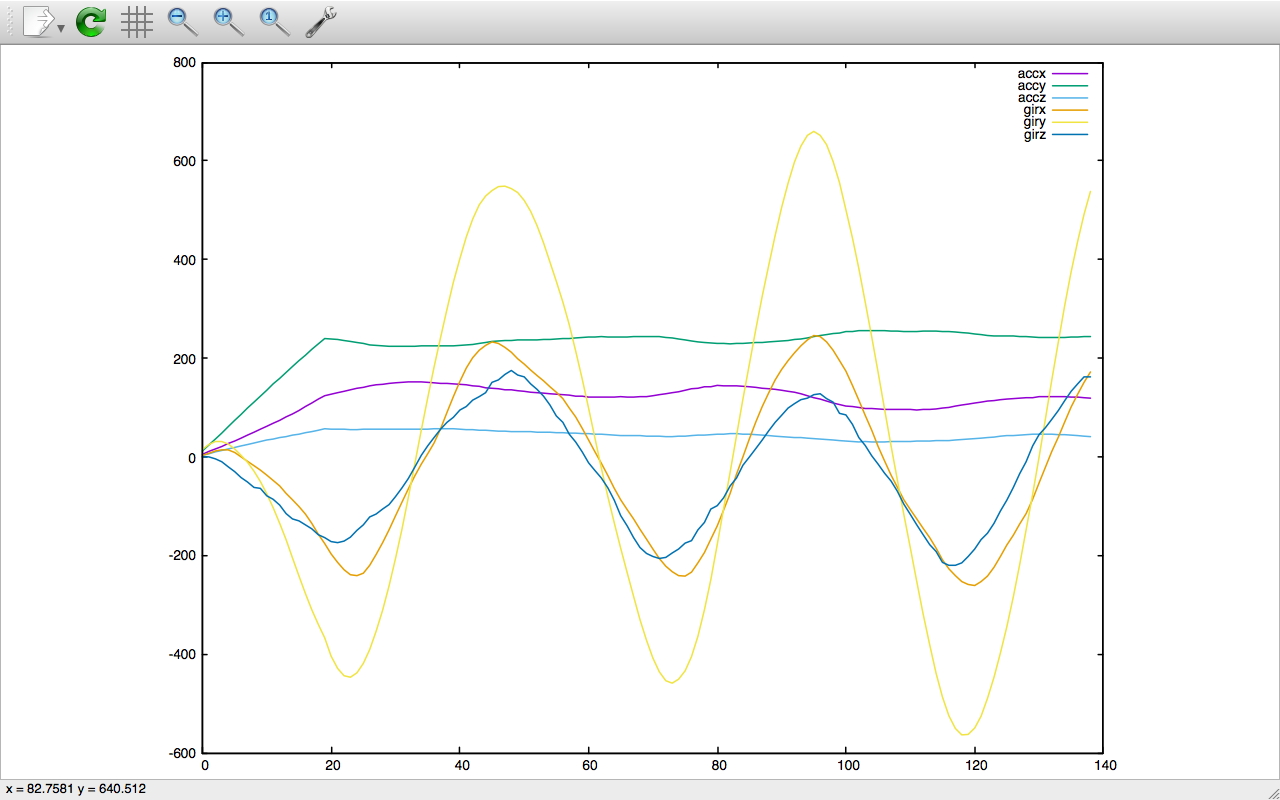
\includegraphics[width=0.9\columnwidth]{img/20}
\caption{Data from the device after preprocessing.}
\label{fig:figure3}
\end{figure}

\subsubsection{Evaluation}
For the actual processing and gesture recognition, we use a sliding window approach on the time series data we receive.
The window is of size 50, hence it will evaluate a sequence of 50 movement instances in a sequence,
every instance consisting of 6 values.
The window is able to capture a period of time of about 2 seconds, as the sampling rate of the device is about 25 Hz.
We organized known gestures in a very large training set, each individual gesture stored as a list of 50 * 6 values plus an identifier, in a way that every gesture will be compatible with the sliding window. 
The training data set in the final version of the project reached more than 500 entries in total.
We use Weka 3.6 to evaluate newly received data using a BayesNet classifier and comparing it to the training set. 
This resulted as the most accurate classifier for our model, giving up to 100\% accuracy when testing it.
The evaluation of the gesture is performed every 10 * 6 new values received.

\subsection{Technical challenges}
\todo{maybe move this part to discussion?}
One of the hardest challenges encountered during the implementation of the system was the interaction with bluetooth and the desktop application for gesture recognition.
The application was programmed in Java, so that it was possible to use the Weka libraries or the gesture evaluation.
We used the BlueCove Java library to build a bluetooth interface \cite{bluecove} \todo{cite bluecove http://bluecove.org/ } in lack of a better alternative.
This library has no longer been updated after 2008, and has some compatibility issues with modern operating systems and java versions.
In particular, OS X deprecated functions that were required for some of the library functionalities after the release of OS X 10.8 in 2012.
Also the library is bound to work in 32 bit mode, which is not supported for java sdk 1.8 nor 1.7.
The only way to make it work was then to downgrade the application to use Java 6.








